% Figure 2: exact multi-token recovery, same layer vs early target, seven model x item-set cells.
% Numbers (majority-of-8 exact rate, 95% item bootstrap) verified from:
%   runs/w3_B_x3i3_14b_ans_L32, runs/w3_A_x3i3_14b_ans_L32 (originals), runs/w5_fresh_14b_{B,A}_x3i3_L32 (fresh),
%   runs/w5_8b_{B,A}_x3i3_L29 (8B, block 8), runs/w3_A_x3i3_1p7b_ans_L22 (1.7B, block 8).
\documentclass[10pt,border=2pt]{standalone}
\usepackage{newtxtext}
\usepackage[T1]{fontenc}
\usepackage{pgfplots}
\pgfplotsset{compat=1.18}
\usetikzlibrary{patterns}
\definecolor{wblue}{HTML}{0072B2}
\definecolor{worange}{HTML}{E69F00}
\begin{document}
\small
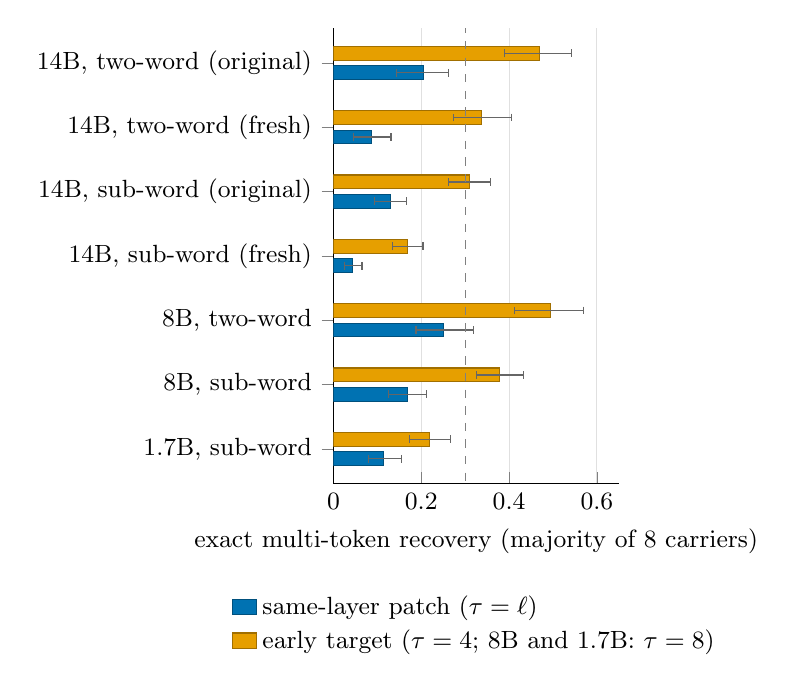
\begin{tikzpicture}
\begin{axis}[
  xbar, width=2.05in, height=2.9in,
  xmin=0, xmax=0.65,
  xlabel={exact multi-token recovery (majority of 8 carriers)},
  xlabel style={font=\small},
  tick label style={font=\small},
  ytick=data,
  yticklabels={{14B, two-word (original)},{14B, two-word (fresh)},{14B, sub-word (original)},{14B, sub-word (fresh)},{8B, two-word},{8B, sub-word},{1.7B, sub-word}},
  y dir=reverse,
  bar width=5pt,
  enlarge y limits=0.09,
  legend style={at={(0.5,-0.22)},anchor=north,font=\small,draw=none,fill=white,legend cell align=left,legend columns=1},
  legend image code/.code={\draw[#1] (0cm,-0.1cm) rectangle (0.3cm,0.1cm);},
  axis x line*=bottom, axis y line*=left,
  xmajorgrids, grid style={black!12},
  error bars/x dir=both, error bars/x explicit,
  error bars/error bar style={black!60,line width=0.5pt},
  error bars/error mark options={rotate=90,mark size=1.4pt,black!60},
]
% same layer
\addplot[fill=wblue,draw=wblue!70!black] coordinates {
 (0.206,0) -= (0.063,0) += (0.057,0)
 (0.086,1) -= (0.040,0) += (0.045,0)
 (0.129,2) -= (0.035,0) += (0.038,0)
 (0.044,3) -= (0.018,0) += (0.021,0)
 (0.250,4) -= (0.062,0) += (0.069,0)
 (0.168,5) -= (0.042,0) += (0.044,0)
 (0.115,6) -= (0.036,0) += (0.040,0)
};
% early target
\addplot[fill=worange,draw=worange!70!black] coordinates {
 (0.469,0) -= (0.080,0) += (0.074,0)
 (0.337,1) -= (0.063,0) += (0.069,0)
 (0.310,2) -= (0.047,0) += (0.047,0)
 (0.169,3) -= (0.034,0) += (0.035,0)
 (0.494,4) -= (0.082,0) += (0.075,0)
 (0.379,5) -= (0.053,0) += (0.053,0)
 (0.219,6) -= (0.046,0) += (0.047,0)
};
\legend{same-layer patch ($\tau=\ell$), early target ($\tau=4$; 8B and 1.7B: $\tau=8$)}
\draw[dashed,black!50] (axis cs:0.30,-0.6) -- (axis cs:0.30,6.6);
\end{axis}
\end{tikzpicture}
\end{document}
